% $Id$

The Laser Interferometric Gravitational Wave Observatory (LIGO)\cite{barish}
has completed three science data taking runs. Analysis of the data for
gravitational waves from coalescing compact binaries has been completed for
the first two runs\cite{bns1,bns2} and is in progress for the third run. Two
of the target populations in these searches are binary neutron
stars\cite{300yrs} and binary black hole MACHOs\cite{sammacho,nakamura}. For
these low mass systems, which have component massed below $3 M_\odot$, the
waveforms of the gravitational radiation emitted are well
known\cite{bdiww,biww}.  Matched filtering is a common and effective technique
for extracting known signals from noise\cite{wz}. We have implemented a
matched filter search gravitational wave interferometer data in the package
\emph{findchirp} which can be found in the LIGO Algorithm Library
(LAL)\cite{lal}.

We describe in detail the algorithms used in findchirp. In section
\ref{s:conventions} we define the conventions that are used for analysis
quantities; in particular the definition of the Fourier transform and the
power spectral density. Section \ref{s:waveforms} gives a brief description of
the the waveforms used and section \ref{s:matchedfilter} describes the
implementation of the matched filter.  Spurious noise may cause the output of
the matched filter to be large and so in section \ref{s:chisq} we describe our
implementation of the $\chi^2$ time--frequency discriminator proposed in
in~\cite{allen}. Section \ref{s:practical} contains details of the aspects of
the search particular to our implementation such as the computation of the
inverse power spectrum and the trigger selection algorithm. This is followed
by a brief conclusion which summarized the methods used and outlines some
future directions for improvement.

%%%%%%%%%%%%%%%%%%%%%%%%%%%%%%%%%%%%%%%%%%%%%%%%%%%%%%%%%%%%%%%%%%%%%%%%%%%%%%%
\section{Conventions}
\label{s:conventions}

The raw (uncalibrated) output of the detector is denoted $v(t)$. In order to
construct a digital matched filter, we sample the output at $N$ consecutive
points with sampling interval $\Delta t$, that is $v_j \equiv v(t_j)$ where
$t_j = j\Delta t$. We reserve the subscript $j$ for discretely sampled time
domain quantities and the subscript $k$ for discretely sampled frequency
domain quantities. For a frequency domain quantity $v(f_k)$ denotes the
value quantity samples at a particular frequency $f_k$ whereas $v_k = v(f_k)
/ \Delta t$ denotes the same quantity divided by the sampling interval.

\subsection{The Fourier Transform}
\label{ss:ftconv}

We define the forward Fourier transform $\tilde{v}(f)$ of a time domain
quantity $v(t)$ to be
\begin{equation}
\label{eq:ft}
\tilde{v}(f)=\int_{-\infty}^\infty dt\,v(t)\, e^{- 2 \pi i f t}
\end{equation}
and the inverse Fourier transform to be 
\begin{equation}
\label{eq:ift}
v(t)=\int_{-\infty}^\infty df\,\tilde{v}(f)\, e^{2 \pi i f t}.
\end{equation}

For the $N$ sample points $v_j$ we may estimate the Fourier transform at 
$N + 1$ samples in the range $[-f_n,f_n]$, where $f_n = 1/(2\Delta t)$ is the
Nyquist critical frequency, by
\begin{equation}
\tilde{v}(f_k) \approx \sum_{j=0}^{N-1} \Delta t\, h(t_j) e^{-2 \pi i f_k t_j}
= \Delta t \sum_{j=0}^{N-1} v_j e^{-2 \pi i j k / N}.
\end{equation}
There are only $N$ independent values of $\tilde{v}(f_k)$ as the extreme
values of $k$ correspond to the upper and lower limits of the Nyquist
frequency range and are equal. The discrete Fourier transform is the defined
to be\cite{T010095}
\begin{equation}
\tilde{v}_k = \sum_{j=0}^{N-1} v_j e^{-i 2 \pi j k / N}.
\end{equation}
We may estimate the discrete inverse Fourier transform from \ref{eq:ift} using
\begin{equation}
\Delta f = f_{k+1} - f_k = \frac{k+1}{N\Delta t} - \frac{k}{N\Delta t} =
\frac{1}{N\Delta t}
\end{equation}
which gives
\begin{equation}
v(t_j) \approx \sum_{k=0}^{N-1} \tilde{v}(f_k) e^{2 \pi i f_k t_j / N} \Delta f
= \frac{1}{N} \sum_{k=0}^{N-1} \tilde{v}_k e^{2 \pi i j k / N}.
\end{equation}

\subsection{Power Spectral Densities}
\label{ss:psdconv}

Consider a signal $n(t)$ containing Gaussian noise and dimensions $U$, which
may be voltage, strain, etc. We define the one sided power spectral density,
$S(|f|)$, of this signal by the equation
\begin{equation}
\left\langle\tilde{n}(f) \tilde{n}^\ast(f')\right\rangle = 
\frac{1}{2}\ospsd\delta(f-f)
\end{equation}
which has units of $\mathrm{time}\times U^2$. For discretely sampled 
quantities we have
\begin{equation}
\left\langle\tilde{n}(f_k) \tilde{n}^\ast(f_{k'})\right\rangle = 
\frac{1}{2}\ospsd\delta(f_k-f_{k'})
\end{equation}
which gives
\begin{equation}
\label{eq:psddef}
\left\langle\tilde{n}_k \tilde{n}_{k'}^\ast\right\rangle = 
\frac{N}{2\Delta t}\ospsd\delta_{kk'}
\end{equation}
which defines \ospsd in terms of the discrete frequency domain quantities.
The definition in equation \ref{eq:psddef} is equivalent to
\begin{equation}
\ospsd = \left\{
\begin{array}{ll}
\frac{\Delta t}{N} | \tilde{n}_0 |^2 & k = 0, \\
\\
\frac{\Delta t}{N} \left[ | \tilde{n}_k |^2 + | \tilde{n}_{N-k} |^2 \right] &
k\neq 0.
\end{array}
\right.
\end{equation}

%%%%%%%%%%%%%%%%%%%%%%%%%%%%%%%%%%%%%%%%%%%%%%%%%%%%%%%%%%%%%%%%%%%%%%%%%%%%%%%
\section{Waveforms from inspiraling compact binaries}
\label{s:waveforms}

Although the binary systems are expected to be highly eccentric and widely
separated when they form\cite{bkb}, the emission of gravitational radiation at
twice the orbital frequency of the binary system causes the orbit to
circularize much faster than it shrinks\cite{peters}. By the time the
frequency of the gravitational radiation enters the sensitive band of the 
detector the orbit is nearly circular, so we neglect eccentricity in the
template waveforms. The effect of spin on the detectability of the waveforms
is not expected to be a significant for low mass binaries\cite{apos} and
neglect it in the templates used here.

We use restricted post-Newtonian (PN) waveforms to construct the filters. The
amplitude evolution is computed from the quadrupole-formula\cite{petersmath}
and the phase evolution is computed to second PN order ($\mathcal{O}(v/c)^4$
where $v$ is the orbital velocity).  For a binary system (circular orbits, no
spin) with masses $m_1$ and $m_2$ solar masses the gravitational wave strain
is
\begin{equation}
h(t) = \frac{1\,\mathrm{Mpc}}{\mathcal{D}}\left(F_{+}h_{+}(t) +
F_{\times}h_{\times}(t)\right),
\end{equation}
where $\mathcal{D}$ is the actual distance to the chirp in Mpc. $h_{+}(t)$
and $h_{\times}(t)$ are the two polarizations of the gravitational wave signal
and $F_{+}$ and $F_{\times}$ are the detector beam pattern functions. The
``$+$'' (plus) polarization is given by
\begin{equation}
h_{+}(t) = -\frac{1 + \cos^2 i}{2}\,h_c(t)
\end{equation}
and the ``$\times$'' (cross) polarization is given by
\begin{equation}
h_{\times}(t) = -\cos i\,h_s(t).
\end{equation}
where $i$ is the inclination angle (radians) of the angular momentum axis
relative to the line-of-sight. The waveforms $h_c(t)$ and $h_s(t)$ are referred
to as the cosine and sine polarizations of the inspiral signal~\cite{biww}.

The template waveforms $h_c(t)$ and $h_s(t)$ are computed for a binary
system that is {\it optimally oriented}. An optimally oriented binary system
lies on the $z$-axis with its orbital plane parallel to the $x$-$y$ plane,
which is defined by the arms of the interferometer. The detector has a
non-uniform response over the sky due to its quadrupolar antenna pattern,
given by $F_\pm$. If the source is not optimally oriented (i.e., not on the
$z$-axis or the orbital plane is tipped), then the effective distance will be
greater than the source-detector distance. Since the search code records the
effective distance to a trigger, when we discuss distances to candidate events
found by the search code we always quote effective distance, that is, distance
to an optimally oriented event.

Since the matched filter is performed in the frequency domain, we use the
stationary phase approximation to the Fourier transform of the 2~PN
waveform\cite{poissonwill}. The stationary phase approximations to the Fourier
transforms of $h_c(t)$ and $h_s(t)$ are given by
\begin{eqnarray}
\label{eq:spcos}
\tilde{h}_c(f)&=&\frac{2T_\odot c}{1\,\mathrm{Mpc}}
\left(\frac{5\mu}{96M_\odot}\right)^\frac{1}{2}
\left(\frac{M}{\pi^2M_\odot}\right)^\frac{1}{3}%\\
%&&\quad\quad\times 
f^{-\frac{7}{6}}\,T_\odot^{-\frac{1}{6}}\,
e^{i\Psi(f;M,\eta)},\\%\nonumber \\
\label{eq:hsorthog}
\tilde{h}_s(f)&=&i\tilde{h}_c(f),
\end{eqnarray}
where $f$ is the gravitational wave frequency in Hz, $M = m_1+m_2$ 
is the total mass of the binary, $\mu = m_1 m_2 / M$ is the reduced mass and
$\eta = \mu/M$.  Note that $\tilde{h}_{c,s}(f)$ have dimensions of 1/Hz.  The
instrument strain per Hz, $\tilde{h}(f)$, is obtained from a linear
superposition of $\tilde{h}_{c,s}(f)$ in exactly the same way as $h(t)$ is
obtained from $h_{c,s}(t)$. The phase evolution to 2~PN order is given by
\begin{eqnarray}
\Psi(f;M,\eta)&=&2\pi ft_c-2\phi_c-\pi/4\nonumber\\
&&+\frac{3}{128\eta}\biggl[x^{-5}+
\left(\frac{3715}{756}+\frac{55}{9}\eta\right)x^{-3}
-16\pi x^{-2}\nonumber\\
&&+\left(\frac{15\,293\,365}{508\,032}+\frac{27\,145}{504}\eta
+\frac{3085}{72}\eta^2\right)x^{-1}\nonumber\biggr],
\end{eqnarray}
where $x=(\pi MfT_\odot/M_\odot)^{1/3}$, the coalescence phase
$\phi_c$ is determined by the binary ephemeris, and the coalescence
time $t_c$ is the time at which the bodies collide.  The chirps
$\tilde{h}_c$ and $\tilde{h}_s$ are given $\phi_c=0$ and
$\phi_c=-\pi/4$, respectively. The validity of the stationary phase
approximation for inspiral templates is well established\cite{spvalid}.

The 2~PN waveform is a sweeping sinusoid which is computed from a specified 
low frequency cutoff which is chosen based on the characteristic noise in the
detector. It sweeps through the sensitive band of the detector with increasing
frequency and amplitude.  The upper frequency cutoff of the waveform is
determined by the frequency at which the post-Newtonian approximation breaks
down and we no longer trust the waveforms. For post-Newtonian chirps computed
in the time domain, the frequency at which the frequency evolution becomes
non-monotonic is a good indication of this.  In the stationary phase
approximation there is no equivalent measure of the breakdown.  Therefore to
set a high frequency cutoff for the inspiral waveforms, we choose the
frequency of the Schwartzchild innermost stable orbit (ISCO). This can be
computed exactly and is given by
\begin{equation}
f_{\mathrm{max}} = \left( 6M\pi\sqrt{6}T_\odot \right)^{-1}\,\mathrm{Hz}
\label{eq:isco}
\end{equation} where $M$ is the total mass of the binary system in solar
masses. Since the ISCO frequency is currently not known for a pair of
comparably massive objects, it is something of a kludge to use this, however
we find in practice that this yields a maximum frequency which is close to that
given by the frequency at which the time domain waveforms are cut off.  The
upper frequency cutoff for the waveform of a $2\times 1.4 \> M_\odot$ binary
system is thus $1570$~Hz.

%%%%%%%%%%%%%%%%%%%%%%%%%%%%%%%%%%%%%%%%%%%%%%%%%%%%%%%%%%%%%%%%%%%%%%%%%%%%%%%
\section{The matched filter}
\label{s:matchedfilter}

The dimensionless strain $h(t)$ of the gravitational wave produces a
differential change $\Delta L(t)=L h(t)$ in the lengths of the two
perpendicular interferometer arms, where $L$ is the average arm length.  In
addition the gravitational wave signal that we wish to detect the
interferometer output contains noise, $n(t)$. We assume that the noise samples
are drawn from a stationary Gaussian distribution, though there may be
correlations among the noise events (colored noise). The noise correlations
may be expressed in terms of the one-sided noise power spectral density,
\ospsd, defined in equation [\ref{eq:psddef}]. The (calibrated) detector
output is $s(t) = h(t) + n(t)$.  Our problem is to detect the presence of a
gravitational wave signal $h(t)$ in the detector output $s(t)$.

\subsection{The maximum likelihood receiver}
\label{ss:maxrec}

A comprehensive discussion of the statistical theory of signal detection can
be found in~\cite{wz} and in the context of binary inspiral
in~\cite{finn,finnchernoff}. The reception process is simply the construction
of some statistic of the data followed by a test of the hypotheses ``there is
a signal present in the data'' and ``there is no signal present in the data.''
When these hypothesis are assumed to be mutually exclusive, the reception
process reduces to the comparison of the statistic with some pre-assigned
threshold. 

As described in section \ref{s:waveforms}, the gravitation radiation from a
binary inspiral is a linear combination of two possible orbital phases,
$h_{+}$ and $h_{\times}$ at a physical distance $\mathcal{D}$. This means that
the signal that we wish to detect, $h(t)$, is known up to an arbitrary phase
$\theta$ and amplitude $A$,
\begin{equation}
h(t) = A \cos \theta h_c(t) + A \sin \theta h_s(t)
\end{equation}
Here we review the construction of a statistic which is optimal for
signals which are known up to an arrival time and phase which are to be
determined.

\textcolor{red}{Add section on statistical theory of matched filtering from
thesis.} We define an inner product $(\cdot|\cdot)$ by
\begin{equation}
\label{eq:innerproduct}
  (a\mid b) \equiv \int_{-\infty}^\infty df\,
  \frac{\tilde{a}^\ast(f)\tilde{b}(f)+\tilde{a}(f)\tilde{b}^\ast(f)}
       {S_h(|f|)}.
\end{equation}

The sine and cosine polarizations of the inspiral signal are orthogonal,
$\left(h_c\mid h_s\right) = 0$. We define the normalization constant
$\sigma^2$ to be
\begin{equation}
\sigma^2 = \left(h_c\mid h_c\right) = \left(h_s\mid h_s\right).
\end{equation}

The inspiral signals that we wish to receive are much shorter than the
observation time, and we do not know when the signals occur. We wish not only
to detect these signals, but also to measure their arrival time. To do so, we
construct the time series
\begin{equation}
\label{eq:xcts}
x(t) = 2 \int_{-\infty}^{\infty}df\,e^{2\pi i f t} 
\frac{\tilde{s}(f) \tilde{h_c}^\ast(f)}{S_n\left(\left|f\right|\right)}
\end{equation}
and
\begin{equation}
\label{eq:ycts}
y(t) = 2 \int_{-\infty}^{\infty}df\,e^{2\pi i f t} 
\frac{\tilde{s}(f) \tilde{h_s}^\ast(f)}{S_n\left(\left|f\right|\right)}.
\end{equation}
For each observation period, we construct the statistic
\begin{equation}
\rho(t) = \frac{1}{\sigma}\sqrt{x^2(t) + y^2(t)}
\end{equation}
and threshold on this statistic, which we call the signal-to-noise ratio
(SNR).

Since the chirp waveforms are are real time series, we have $h(f) =
h^\ast(-f)$ and the inner product (\ref{eq:innerproduct}) becomes
\begin{equation}
\left(a\mid b\right) = 2 \int_{-\infty}^{\infty}df\,
\frac{\tilde{a}^\ast(f)\tilde{b}(f)}{S_h\left(\left|f\right|\right)}
\end{equation}
so the normalization constant $\sigma$ is
\begin{equation}
\label{eq:sigmasqcts}
\sigma^2 = 2 \int_{-\infty}^{\infty}df\,
\frac{\tilde{h_c}^\ast(f)\tilde{h_c}(f)}{S_h\left(\left|f\right|\right)} 
= 2 \int_{-\infty}^\infty 
\frac{\tilde{h_s}^\ast(f)\tilde{h_s}(f)}{S_h\left(\left|f\right|\right)}.
\end{equation}
The filter that we have constructed is normalized according to the convention
of Cutler and Flanagan \cite{cutflan}, so that in the case when the detector
output is Gaussian noise, the filter output averaged over an ensemble of
detectors with different realizations of the noise is
$\left\langle \rho^2 \right\rangle = \left\langle x^2 + y^2 \right\rangle = 2$.

\subsection{Construction of the digital filter using stationary phase chirps}
\label{ss:digitalfilter}

Since the two chirp waveforms $\tilde{h_c}$ and $\tilde{h_s}$ are 
orthogonal, it is possible to increase the efficiency of the algorithm by
constructing the single time $\rho(t)$ directly using a single complex inverse
FFT rather than computing it from $x(t)$ and $y(t)$ which requires two real
inverse FFTs. We may further increase efficiency when using stationary phase
chirps by dividing the filter into a part that depends on the data and a part
that depends only on the template parameters. In this section we describe the
construction of the digital filter used in findchirp, which uses these two 
methods. Consider the discrete form of equation (\ref{eq:xcts})
\begin{eqnarray}
\label{eq:xdisc}
x_j &=& \frac{2}{\sigma} \frac{1}{N\Delta t} \sum_{k=0}^{N-1} e^{2\pi ijk/N} 
\frac{\tilde{s}(f_k) \tilde{h}_{c}^\ast(f_k)}{\ospsd} \\
&=&
\frac{2}{\sigma} \frac{\Delta t}{N} \sum_{k=0}^{N-1} e^{2\pi ijk/N} 
\frac{\tilde{s}_k \tilde{h}_{ck}^\ast} {\ospsd}
\end{eqnarray}
where we have used $\tilde{s}(f_k) = \Delta t\, \tilde{s}_k$ and
$\times{h}_c(f_k) \equiv \Delta t\, \tilde{h}_{ck}$. From equation
(\ref{eq:ycts}) we obtain
\begin{equation}
\label{eq:ydisc}
y_j = \frac{2}{\sigma} \frac{\Delta t}{N} \sum_{k=0}^{N-1} e^{2\pi ijk/N} 
\frac{\tilde{s}_k \tilde{h}_{sk}^\ast} {\ospsd}
\end{equation}
The normalization constant $\sigma^2$ defined in equation
(\ref{eq:sigmasqcts}) is
\begin{eqnarray}
\label{eq:sigmasqdisc}
\sigma^2 &=& 2 \frac{1}{N\Delta t} \sum_{k=0}^{N-1}
\frac{\tilde{h}_{c}(f_k)\tilde{h}_{c}^\ast(f_k)}{\ospsd} 
=
2 \frac{\Delta t}{N} \sum_{k=0}^{N-1}
\frac{\tilde{h}_{ck}\tilde{h}_{ck}^\ast}{\ospsd} \\
&=&
4 \frac{\Delta t}{N} \sum_{k=0}^{N/2}
\frac{\tilde{h}_{ck}\tilde{h}_{ck}^\ast}{\ospsd}
\end{eqnarray}
Now we may use the fact that $s(t)$ is a real signal and so $\tilde{s}(f) = 
\tilde{s}(-f)^\ast$ to write equation the cosine phase of the filter 
(\ref{eq:xdisc}) as
\begin{eqnarray}
x_j &=& 
\frac{2}{\sigma}\frac{\Delta t}{N}
\left[
  \sum_{k=N/2}^{N-1} e^{2\pi ijk/N} 
  \frac{\tilde{s}_k \tilde{h}_{ck}^\ast}{\ospsd}
  +
  \sum_{k=0}^{N/2} e^{2\pi ijk/N} 
  \frac{\tilde{s}_k \tilde{h}_{ck}^\ast}{\ospsd}
\right] \\
&=& 
\frac{2}{\sigma}\frac{\Delta t}{N}
\left[
  \sum_{k=0}^{N/2} e^{-2\pi ijk/N} 
  \frac{\tilde{s}_k^\ast \tilde{h}_{ck}}{\ospsd}
  +
  \sum_{k=0}^{N/2} e^{2\pi ijk/N} 
  \frac{\tilde{s}_k \tilde{h}_{ck}^\ast}{\ospsd}
\right] \\
&=&
\frac{2}{\sigma}\frac{\Delta t}{N}(Q_j^\ast + Q_j)
\end{eqnarray}
where
\begin{equation}
\label{eq:Qdef}
Q_j = \sum_{k=0}^{N/2} e^{2\pi ijk/N} 
  \frac{\tilde{s}_k \tilde{h}_{ck}^\ast}{\ospsd}.
\end{equation}
The sine phase of the filter (\ref{eq:ydisc}) can be written as
\begin{eqnarray}
\label{eq:yinter}
y_j &=&
\frac{2}{\sigma}\frac{\Delta t}{N}
\left[
  \sum_{k=N/2}^{N-1} e^{2\pi ijk/N} 
  \frac{\tilde{s}_k \tilde{h}_{sk}^\ast}{\ospsd}
  +
  \sum_{k=0}^{N/2} e^{2\pi ijk/N} 
  \frac{\tilde{s}_k \tilde{h}_{sk}^\ast}{\ospsd}
\right] \\
&=& 
\frac{2}{\sigma}\frac{\Delta t}{N}
\left[
  \sum_{k=0}^{N/2} e^{-2\pi ijk/N} 
  \frac{\tilde{s}_k^\ast \tilde{h}_{sk}}{\ospsd}
  +
  \sum_{k=0}^{N/2} e^{2\pi ijk/N} 
  \frac{\tilde{s}_k \tilde{h}_{sk}^\ast}{\ospsd}
\right]
\end{eqnarray}
Using (\ref{eq:hsorthog}), equation (\ref{eq:yinter}) becomes
\begin{eqnarray}
y_j &=& 
\frac{2}{\sigma}\frac{\Delta t}{N}
\left[
  \sum_{k=0}^{N/2} e^{-2\pi ijk/N} 
  \frac{\tilde{s}_k^\ast i\tilde{h}_{ck}}{\ospsd}
  +
  \sum_{k=0}^{N/2} e^{2\pi ijk/N} 
  \frac{\tilde{s}_k (-i)\tilde{h}_{ck}^\ast}{\ospsd}
\right] \\
&=& 
\frac{-2i}{\sigma}\frac{\Delta t}{N}
\left[
  - \sum_{k=0}^{N/2} e^{-2\pi ijk/N} 
  \frac{\tilde{s}_k^\ast \tilde{h}_{ck}}{\ospsd}
  +
  \sum_{k=0}^{N/2} e^{2\pi ijk/N} 
  \frac{\tilde{s}_k \tilde{h}_{ck}^\ast}{\ospsd}
\right] \\
&=& 
\frac{2}{\sigma}\frac{\Delta t}{N}i(Q_j^\ast - Q_j).
\end{eqnarray}
This the outputs of the filter for the two phases are
\begin{equation}
x_j = \frac{4}{\sigma} \Re z_j,
\quad\mathrm{and}\quad
y_j = \frac{4}{\sigma} \Im z_j.
\end{equation}
The quantity $z_j$ is defined to be \textcolor{red}{(check factors 
of $\Delta t$ so $z$ matches S2 paper.)}
\begin{equation}
\label{eq:zdef}
z_j = \frac{\Delta t}{N}\sum_{k=0}^{N/2} e^{2\pi ijk/N} 
\frac{\tilde{s}_k \tilde{h}_{ck}^\ast}{\ospsd} 
= \frac{\Delta t}{N}\sum_{k=0}^{N-1} e^{2\pi ijk/N} \tilde{z}_k
\end{equation}
where
\begin{equation}
\label{eq:ztildedef}
\tilde{z}_k = \left\{
\begin{array}{ll}
\frac{\tilde{s}_k \tilde{h}_{ck}^\ast}{\ospsd} 
  \quad\quad & 0 < k < \frac{N}{2},\\
\\
0 & \mathrm{otherwise}.
\end{array}
\right.
\end{equation}
We can now compute the square of the signal-to-noise ratio
\begin{equation}
\rho^2(t_j) = x_j^2 + y_j^2 = \frac{16}{\sigma^2}|z_j|^2
\end{equation}
by a single complex inverse Fourier transform and threshold on 
$\rho^2 \ge \rho^2_\ast$.  Since we choose the 2~PN stationary phase template
chirp $\tilde{h}_c(f)$ to be at a canonical distance of $1$~Mpc, the effective
distance $\mathcal{D}$ to a chirp detected with signal to noise ratio $\rho^2$
is then given by
\begin{equation}
\mathcal{D}\,(\mathrm{Mpc})= \sqrt{\frac{\sigma^2}{\rho^2}}.
\end{equation}

The calibrated detector output is related to the raw detector output by the
detector response function according to
\begin{equation}
\tilde{s}(f) = R(f;t) \tilde{v}(f)
\end{equation}
where $R(f;t)$ is the (complex) response function of the detector at a
specific time $t$\cite{calpaper}. In practice, we compute the uncalibrated
power spectral density $S_v(|f_k|)$ from the raw data and then the calibrated
power spectral density, $\ospsd$, in the denominator of (\ref{eq:zdef}) is
\begin{equation}
\ospsd = |R(f;t)|^2 S_v(|f_k|).
\end{equation}
Further details of the computation of $S_v(|f_k|)$ are given in sections
\ref{ss:psd} and \ref{ss:invspec}.

Typical values of the variance of $v(t)$ for initial LIGO data are $10^3$,
however the response function, $R(f)$, has magnitude $\sim 10^{-22}$ in the
sensitive band of the instrument. Although we only need floating point (4
byte) precision to store the calibrated interferometer data, $\tilde{s}(f)$
and power spectral density, $S_n(|f|)$, the calibrated time domain data bay
overflow the dynamic range of floating point variables. Therefore when we
implement the digital filter, we multiply the response function $R(f)$ by a
scaling variable, $d$, which typically has values of $d = 2^{64}$ for initial
LIGO data, This scales all frequency domain quantities to of order $\sim$ 
unity.  Therefore equation (\ref{eq:zdef}) becomes
\begin{equation}
\label{eq:zdefcal}
z_j = \sum_{k=0}^{N/2} e^{2\pi ijk/N} 
  \frac{dR\tilde{v}_k\, d\tilde{h}_{ck}^\ast}
  {d^2|R|^2S_v\left(\left|f_k\right|\right)}
\end{equation}
and (\ref{eq:sigmasqdisc}) becomes
\begin{equation}
\label{eq:sigmasqdisccal}
\sigma^2 = 4 \frac{\Delta t}{N} \sum_{k=0}^{N/2}
\frac{d^2 \tilde{h}_{ck}\tilde{h}_{ck}^\ast}
{d^2|R|^2S_v\left(\left|f_k\right|\right)}. 
\end{equation}
Notice that we must also multiply the chirp by $d$ so that all the factors of
$d$ cancel in the signal-to-noise ratio, $\rho(t_j)$, and the normalization
constant, $\sigma^2$. In fact this is conventient as it brings the value of
the strain $h_c(f_k)$ to order unity. 

We now return to the definition of $\tilde{h}_{ck}$.  From equation
(\ref{eq:spcos}) we define the dimensionless quantity
\begin{eqnarray}
\label{eq:hck}
d\,\tilde{h}_{ck} &=& \frac{d \tilde{h}_c(f_k)}{\Delta t} \\
&=& 
\frac{2dT_\odot c}{1\,\mathrm{Mpc}}
\left(\frac{5\mu}{96M_\odot}\right)^\frac{1}{2}
\left(\frac{M}{\pi^2M_\odot}\right)^\frac{1}{3}
\left(\frac{T_\odot}{\Delta t}\right)^{-\frac{1}{6}}\\
&&\quad\quad\times
\left( f\,\Delta t \right)^{-\frac{7}{6}}
\exp\,[i\Psi(f_k;M,\eta)], \nonumber \\
&=&
\sqrt{\mathcal{T}(M,\mu)}\left(\frac{k}{N}\right)^{-\frac{7}{6}}
\exp\left[i\Psi\left(f_k;M,\eta\right)\right]
\end{eqnarray}
where $\mathcal{T}(M,\mu)$ is defined to be
\begin{equation}
\mathcal{T}(M,\mu) = \left[
\left(\frac{2dT_\odot c}{1\,\mathrm{Mpc}}\right)
\left(\frac{5\mu}{96M_\odot}\right)^\frac{1}{2}
\left(\frac{M}{\pi^2M_\odot}\right)^\frac{1}{3}
\left(\frac{T_\odot}{\Delta t}\right)^{-\frac{1}{6}}
\right]^2.
\end{equation}
$\mathcal{T}$ is refered to as the \emph{template dependent normalization
constant}. It depends on the masses of the template and as such must be
recomputed once per template. If we substitute equation (\ref{eq:hck}) 
into equation (\ref{eq:sigmasqdisccal}) we obtain
\begin{equation}
\sigma^2 = 4 \frac{\Delta t}{N} \sum_{k=0}^{N/2} \mathcal{T} 
\sum_{k=0}^{N/2} 
\frac{\left({k}/{N}\right)^{-\frac{7}{3}}}
{d^2|R|^2S_v\left(\left|f_k\right|\right)}
= 4 \frac{\Delta t}{N} \mathcal{T} \mathcal{S}
\end{equation}
where $\mathcal{S}$ is defined to be
\begin{equation}
\mathcal{S} = 
\sum_{k=0}^{N/2} 
\frac{\left({k}/{N}\right)^{-7/3}}{d^2|R|^2S_v\left(\left|f_k\right|\right)}.
\end{equation}
$\mathcal{S}$ is refered to as the \emph{segment dependent normalization} and
needs to be computed only once for a given power spectral density.

The signal-to-noise ratio squared is then
\begin{eqnarray}
\rho^2(t_j) &=& 
\frac{16}{\sigma^2}\left(\frac{\Delta T}{N}\right)^2 \mathcal{T} \nonumber \\
&&\quad\quad\times
\left| 
  \sum_{k=0}^{N/2} e^{2\pi ijk/N} 
  \frac{dR\tilde{v}_k (k/N)^{-7/6} e^{-i\Psi(f_k;M,\eta)}}
       {d^2|R|^2 S_v\left(\left|f_k\right|\right)}
\right|^2 
\end{eqnarray}
where $\sigma^2$ is simply
\begin{equation}
\sigma^2 = \frac{4\Delta t}{N} \mathcal{T}\mathcal{S}.
\end{equation}
Let us define $\tilde{q}_k$ by
\begin{equation}
\label{eq:qtildedef}
\tilde{q}_k = \left\{
\begin{array}{ll}
\frac{d\tilde{v}_k (k/N)^{-7/6} e^{-i\Psi(f_k;M,\eta)}}
     {d^2|R|^2S_v\left(\left|f_k\right|\right)} 
  \quad\quad & 0 < k < \frac{N}{2},\\
\\
0 & \mathrm{otherwise}.
\end{array}
\right.
\end{equation}
and $q_j$ as the discrete inverse Fourier transform of $\tilde{q}_k$, then
the signal-to-noise ration squared is
\begin{equation}
\rho^2(t_j) = \frac{16}{\sigma^2}\left(\frac{\delta T}{N}\right)^2 \mathcal{T}
\left|q_j\right|^2
\end{equation}
The computation of $\tilde{q}_k$ can further be split into the template
independent computation of
\begin{equation}
\tilde{F}_k = \frac{d\tilde{v}_k (k/N)^\frac{-7}{6}}
{d^2|R|^2S_v\left(\left|f_k\right|\right)}
\end{equation}
and the computation of
\begin{equation}
\tilde{T}_k = \exp\left[i\Psi(f_k;M,\eta)\right]
\end{equation}
where $\tilde{F}_k$ is called the \emph{findchirp data segment} and 
$\tilde{T}_k$ is called the \emph{findchirp template}, so
\begin{equation}
\tilde{q}_k = \left\{
\begin{array}{ll}
\tilde{F}_k \tilde{T}_k^\ast \quad\quad & 0 < k < \frac{N}{2},\\
\\
0 & \mathrm{otherwise}.
\end{array}
\right.
\end{equation}

In practice we construct the average power spectral density from $m$ data
segments and then this $\ospsd$ to filter each of the $m$ segments for
inspiral signals. Using the above relationships, we only need to compute
$\mathcal{S}$ once per PSD and $\tilde{F}_k$ once per data segment. We can
then store these quantities re-use them, computing $\mathcal{T}$ and
$\tilde{T}_k$ once per template. We also save some computational effort by
computing
\begin{equation}
|q_j|^2_\ast = \rho^2_\ast \left/
\frac{16}{\sigma^2}\left(\frac{\Delta t}{N}\right)^2 \mathcal{T} \right.
\end{equation}
and thresholding on $|q_j|^2 \ge |q_j|^2_\ast$. \textcolor{red}{Note that we
now compute the template normalization correctly for chirps with different
high frequency cutoffs. This needs to be added to this section.}

\section{The $\chi^2$ veto}
\label{s:chisq}

Let $u$ and $v$ be two orthonormal time series representing the two phases of a
binary inspiral signal, $h_c(t_j)$ and $h_s(t_j)$.  We divide these waveforms
into $p$ frequency sub-intervals $\{u_l\}$ and $\{v_l\}$, $l=1\ldots p$ with
\begin{eqnarray}
  (u_l|u_m) &=& \frac{1}{p}\delta_{Lm} \\
  (v_l|v_m) &=& \frac{1}{p}\delta_{Lm} \\
  (u_l|v_m) &=& 0
\end{eqnarray}
with $u=\sum_{l=1}^p u_l$ and $v=\sum_{l=1}^p v_l$.

We then obtain the $2p$ time series $\{X_l\}=(h|u_l)$ and $\{Y_l\}=(h|v_l)$,
where $h$ is the detector output. Notice that  $X=\sum_{l=1}^p X_l=(h|u)$ and
$Y=\sum_{i=l}^p Y_l=(h|v)$ so that $X^2+Y^2=\rho^2$ is the signal to noise
ratio squared. Now, let $\Delta X_l=X_l-X/p$ and $\Delta Y_l=Y_l-Y/p$ and
define
\begin{equation}
  r^2 = \sum_{l=1}^p \bigl\{ (\Delta X_l)^2 + (\Delta Y_l)^2 \bigr\}
\end{equation}
In the presence of Gaussian noise alone, $h=n$, $\chi^2=pr^2$ is chi-squared
distributed with $\nu=2p-2$ degrees of freedom.  Furthermore, if a signal
$s=Au+Bv$ (with signal to noise squared of $\rho^2_{\mathrm{signal}}=A^2+B^2$) 
is present along with Gaussian noise, $h=s+n$, then $\chi^2=pr^2$ is still
chi-squared distributed with $\nu=2p-2$ degrees of freedom.

\subsubsection{Mismatched signal.}
Suppose a signal that is not exactly matched by $u$ or $v$ is present in
the data: $h=Aw$ where $w$ is a normal vector and $A$ is an amplitude.
(Here we assume no noise.)  With no loss of generality, orient $u$ and $v$
such that $(w|v)=0$.  If $w$ is nearly parallel to $u$, separated by some
parameter difference $\delta x^\alpha$ (which is small) then
\begin{equation}
  w \simeq u + u_{,\alpha}\delta x^\alpha 
  + {\textstyle{\frac{1}{2}}}u_{,\alpha\beta}\delta x^\alpha\delta x^\beta
\end{equation}
so
\begin{eqnarray}
  (h|u) &\simeq& A(u + u_{,\alpha}\delta x^\alpha 
  + {\textstyle{\frac{1}{2}}} u_{,\alpha\beta}\delta x^\alpha\delta x^\beta|u)
  \nonumber\\
  &=& A\bigl\{ (u|u) + (u_{,\alpha}|u)\delta x^\alpha
  + {\textstyle{\frac{1}{2}}} (u_{,\alpha\beta}|u)\delta x^\alpha\delta x^\beta
  \bigr\}\nonumber\\
  &=& A\bigl\{ 1 +
  {\textstyle{\frac{1}{2}}} (u_{,\alpha\beta}|u)\delta x^\alpha\delta x^\beta
  \bigr\}
\end{eqnarray}
since $(w|u)$ is a local maximum for $w=u$; thus $(u_{,\alpha}|u)=0$.

Define the parameter space distance
\begin{equation}
  ds^2 = g_{\alpha\beta}\delta x^\alpha\delta x^\beta
  - {\textstyle{\frac{1}{2}}} (u_{,\alpha\beta}|u)\delta x^\alpha\delta x^\beta.
\end{equation}
so $g_{\alpha\beta}=-{\textstyle{\frac{1}{2}}}(u_{,\alpha\beta}|u)$.

Now compute $r^2$.  We can ignore the $v$ terms.  Thus
\begin{eqnarray}
  r^2 &=& \sum_{l=1}^p \bigl[ (h|u_l) - (h|u)/p \bigr]^2 \\
      &=& \sum_{i=l}^p \bigl\{ (h|u_l)^2 - 2(h|u)(h|u_l)/p + (h|u)^2/p^2 \bigr\}
          \\
      &=& \sum_{i=l}^p (h|u_l)^2 - (h|u)^2/p.
\end{eqnarray}
Now $(h|u_l)^2\le(h|h)(u_l|u_l)=(h|h)/p$ so
\begin{eqnarray}
  r^2 &\le& \frac{1}{p}\bigl[ (h|h) - (h|u)^2 \bigr] \\
      &=& \frac{A^2}{p}\bigl[ (w|w) - (w|u)^2 \bigr] \\
      &=& \frac{A^2}{p}\bigl[ 1 - ( 1 - ds^2 )^2 \bigr] \\
      &\simeq& \frac{2A^2ds^2}{p}.
\end{eqnarray}

Therefore, if $h=Aw+n$ where $w$ has a slight mismatch $ds^2=1-(w|u)$, then
$\chi^2=pr^2$ has a non-central chi-squared distribution with $\nu=2p-2$
degrees of freedom and a non-central parameter $\lambda=2A^2ds^2$.

A chi-squared distribution with $\nu$ degrees of freedom has a mean of
$\nu$ and a variance of $2\nu$ in Gaussian noise; hence one often considers
the quantity $\chi^2/\nu$ (which is very close to the $r^2$ statistic) which
would have a unit mean and a variance of two in the presence of Gaussian
noise alone.  A non central chi-squared distribution with $\nu$ degrees of
freedom and non-central parameter $\lambda$ has a mean of $\nu+\lambda$ and
a variance of $2(\nu+\lambda)\times[1+\lambda/(\nu+\lambda)]$.  (The factor
in brackets in the variance is always between 1 and 2, and is not really
important.)  Thus, in this case, the quantity $\chi^2/(\nu+\lambda)$ has
unit mean and variance of between two and four.

While it is possible to construct constant confidence thresholds on the
non-central chi-squared distribution for various signal events, a crude
(but perhaps adequate) prescription would be just to threshold on the
quantity $\chi^2/(\nu+\lambda)$, which is roughly equivalent to thresholding
on $r^2/(1+A^2ds^2/p)$.  (Since the noise is not really Gaussian anyway,
it does not seem important to use the exact result for the non-central
chi-squared distribution, though this could certainly be done.)

In the inspiral analysis performed here, we construct the time series
\begin{equation}
\mathcal{R}^2(t_j) = \frac{r^2(t_j)}{1+\frac{\rho^2(t_j)\,ds^2}{p}}
\label{e:modified-chisq}
\end{equation}
where $ds^2$ is be the maximum mismatch expected for binary inspirals,
$\rho^2$ is the the signal to noise ratio squared of the putative trigger, and
$p$ is the number of frequency bands that were used in constructing the $r^2$
statistic.  When we refer to the vetoing on the $\chi^2$ statistic, we are
thresholding on the value of $\mathcal{R}^2(t_j)$ for an inspiral trigger at
$t_j$. This is the value that is is recorded in the database table
\verb|CHISQ|. The number of frequency bands $p$ is stored in the database
table \verb|CHISQ_DOF|.

The number of frequency bands is chosen to be 8. Increasing the number of
frequency bands increases the computational overhead for the $\chi^2$ veto and
this number was chosen as a compromise between computational and detection
efficiencies. $ds^2 = 0.03$ is set by the template bank mismatch. 


%%%%%%%%%%%%%%%%%%%%%%%%%%%%%%%%%%%%%%%%%%%%%%%%%%%%%%%%%%%%%%%%%%%%%%%%%%%%%%%
\section{Practical details of the implementation}
\label{s:practical}

\subsection{Power Spectral Estimation}
\label{ss:psd}

\subsection{Computation of the inverse power spectrum}
\label{ss:invspec}
Recall that the FFT we use to compute the match filter treats the data as

being periodic and that we had to ignore part of the filter output that was
corrupted due to wraparound of the filter output from the chirp signal. 

As well as the chirp, we are also filtering the data against the inverse power
spectrum. The chirp has a duration that is typically much less than the
length of the data segment. It only corrupts a region that is the length of
the chirp at the start of the data segment. However, in the time domain the
inverse power spectrum is the same length of the data segment. This will cause
the filter output to be corrupted for all times, as it is non-zero over the
entire data segment.

To prevent this, we truncate the inverse power spectrum to a specified length
in the time domain. This has the effect of smoothing out the high $Q$ features
and restricting the corruption of the filter to the part of the data segment
where the power spectrum is non-zero. These regions can then be ignored when
searching for chirps in the filter output.

The parameter that controls the duration of the power spectrum in the time
domain is \texttt{invSpecTrunc} and the algorithm used to perform the
truncation is as follows:
\begin{enumerate}
\item Compute the square root of the inverse power spectrum,
$\sqrt{S^{-1}_v(|f_k|)}$.
\item Set the Nyquist, $k = N/2$ and DC $k = 0$ components of this to zero.
\item Inverse FFT to to obtain the time domain inverse PSD of length $N$
points.
\item Zero the spectrum between the points $j = \mathtt{invSpecTrunc}/2$ and 
$j = N - \mathtt{invSpecTrunc}/2$. This sets the length of the inverse
spectrum in the time domain to be \texttt{invSpecTrunc} points.
\item FFT the time domain quantity back to the frequency domain.
\item Divide by $N$ so that to recover the quantity before the inverse FFT.
\item Square this quantity to recover $S^{-1}_v(|f_k|)$.
\item Set the Nyquist and DC frequencies to zero and zero the inverse power
spectrum below $f_{\mathrm{low}}$.
\end{enumerate}
The strain inverse power spectral density is then computed by
\begin{equation}
S^{-1}_h(|f_k|) = \frac{1}{\left|\mathtt{dynRange} \times R(f_k)\right|^2}
 S^{-1}_v(|f_k|).
\end{equation}
In this analysis we set the length of the inverse power spectrum in the time
domain to 16 seconds.

\subsection{Trigger selection algorithm}
\label{ss:trigger}

The object of the search algorithm is to generate a list of inspiral triggers
from this time series; times at which there may be a binary inspiral signal in
the data stream. The GPS time recorded in the trigger is the coalescence time of
an inspiral signal, which corresponds to the time at which the signal to noise
ratio squared is a maximum, as shown in figure
\ref{f:zero_inject_zoom}.
\begin{figure}[htp]
\begin{center}
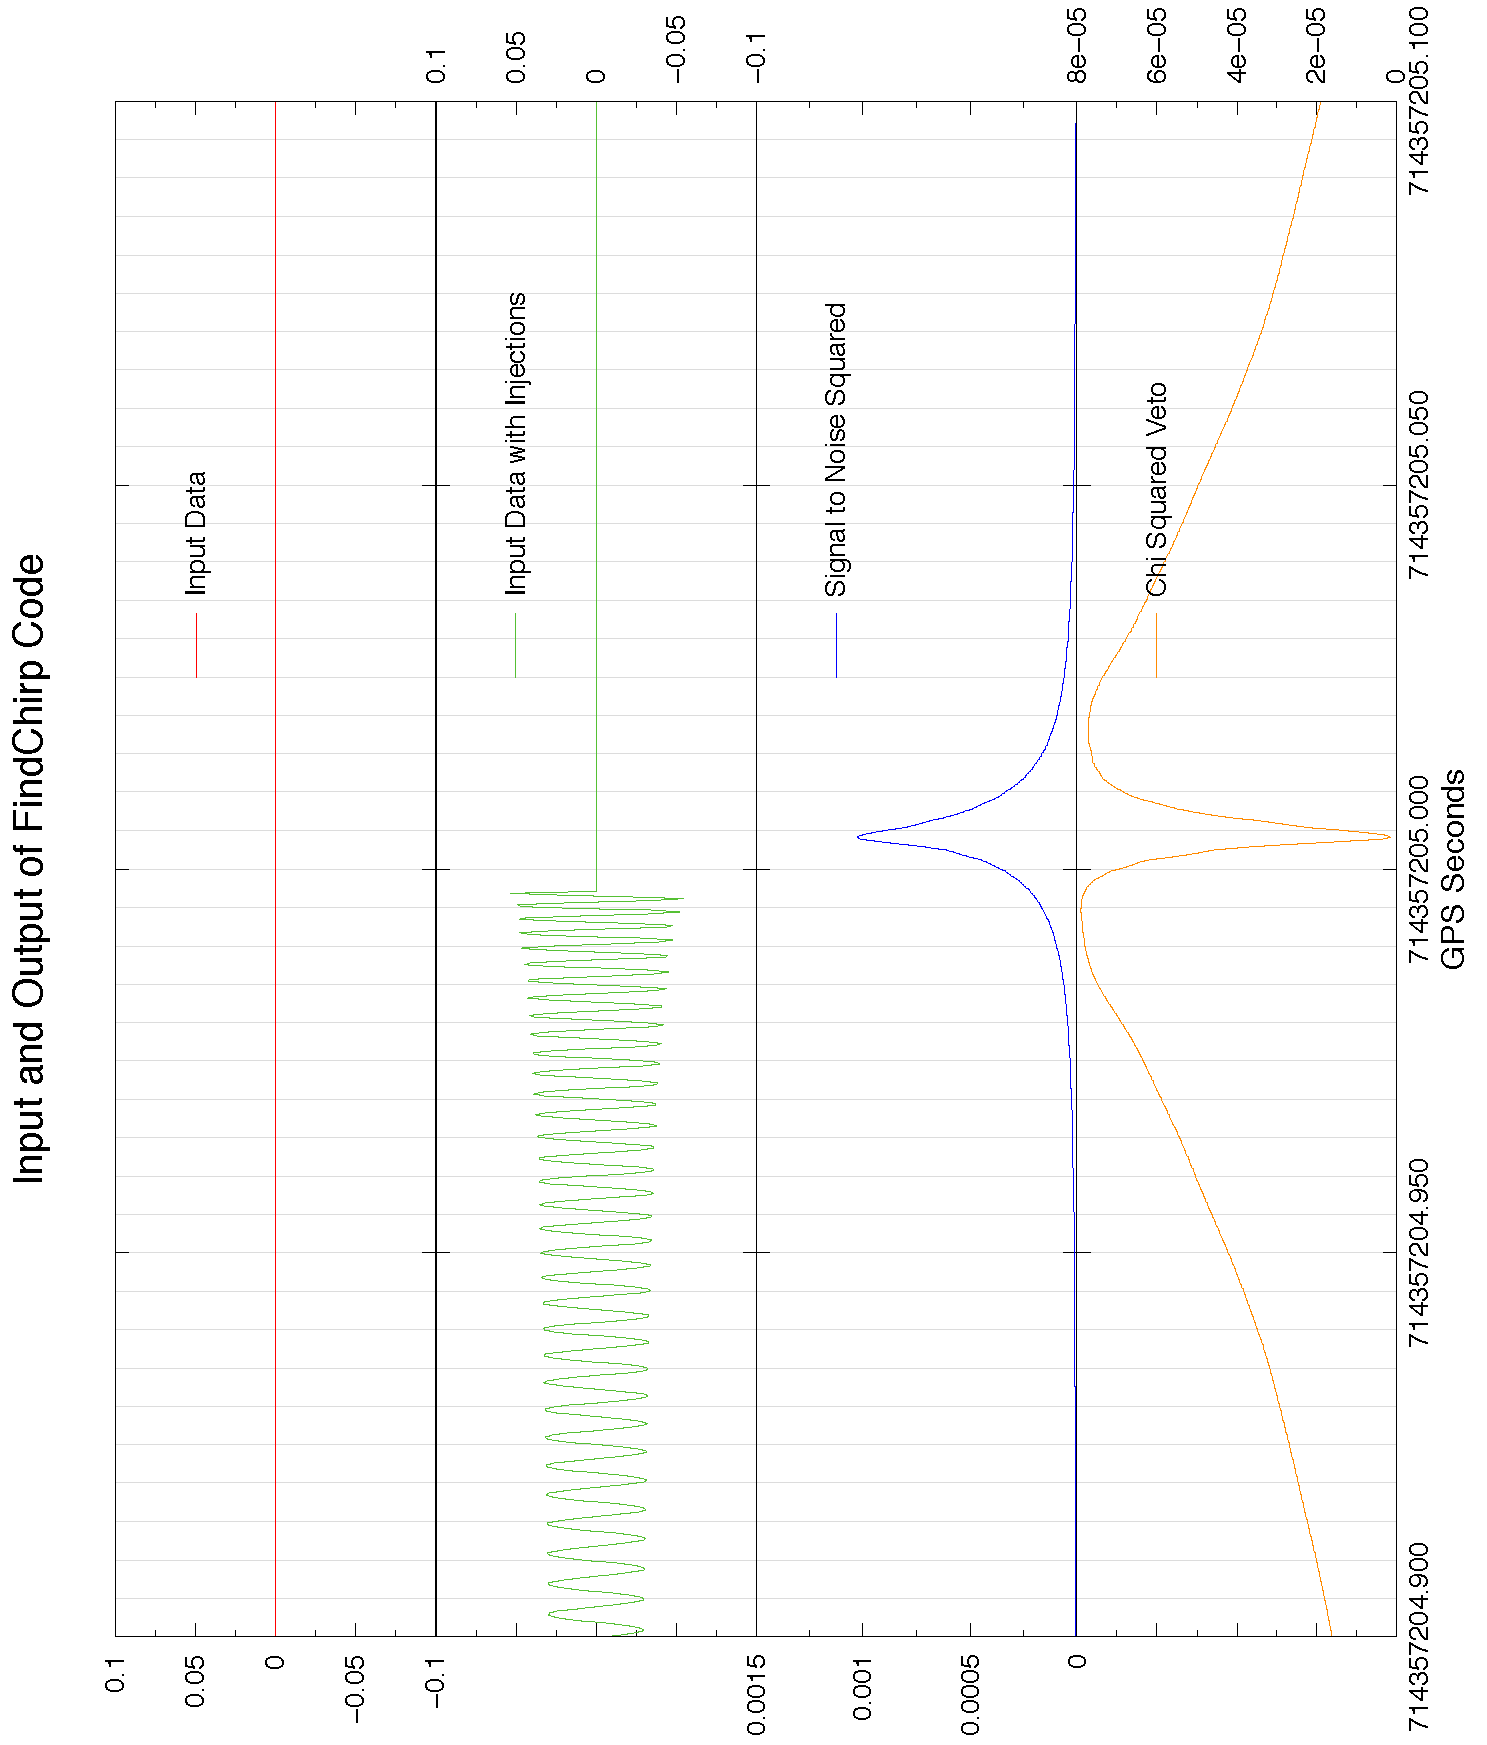
\includegraphics[angle=-90,width=0.75\linewidth]{figures/findchirp/zero_inject_zoom}
\end{center}
\caption{\label{f:zero_inject_zoom}Output time series from the filtering code
for an inspiral chirp in the absence of noise. A $(2.0,2.0)\,m_\odot$ inspiral
chirp is generated using the 2pN time domain waveform generation and injected
into the data. This is filtered using the 2pN stationary phase waveform. The
signal to noise squared and $\chi^2$ time series are shown.  The signal to
noise squared is a maximum at the coalescence time of the \textit{template}
inspiral signal. This occurs slightly after the coalescence time of the
injected signal. The difference in coalescence times is due to the different
methods of generating the chirp signal.
}
\end{figure}
The algorithm to generate triggers is based on the following:
\begin{itemize}
\item The signal to noise ratio of a trigger must exceed some threshold to
distinguish the trigger from background noise in the detector. 

\item The value of the $\chi^2$ statistic for the trigger should be less than
some threshold value $\chi^2_\ast$ to veto triggers that exceed the signal to
noise threshold, but do not have the characteristic waveform of an inspiral
signal (e.g. impulse like events in the data).

\item We do not want to construct triggers from times at which the output
signal to noise time series is corrupted by wrap around from the inspiral
template or the inverse power spectrum.

\item The length of a data segment is greater than the length of a chirp, so
may be multiple chirps in a single segment.
\end{itemize}

Given these requirements, the algorithm for construction of the list of
inspiral triggers is as follows:

\begin{enumerate}

\item Compute the length of the inspiral chirp used as the template
\begin{equation}
t_\mathrm{chirp} = \frac{5m}{256\eta} 
  x^{-8}\left(1 + \alpha x^2 + \beta x^3 + \gamma x^4 \right)
\end{equation}
where
\begin{eqnarray}
x & = & \left(\pi m T_\odot f_{\mathrm{low}}\right)^{\frac{1}{3}}, \\
\alpha & = & \frac{743}{252} + \frac{11}{3}\eta, \\
\beta & = & -\frac{32\pi}{3}, \\
\gamma & = & \frac{3058673}{508032}+\frac{5429}{504}\eta+\frac{617}{71}\eta^2,
\end{eqnarray}
$m$ is the mass of the more massive object and $f_{\mathrm{low}}$ is the low
frequency cutoff of the inspiral template.

\item Since the overlap of the data segments is one half the length of a
segment, set the length of time to ignore at the start and end of the data
segment to be one quarter of the length of a data segment.

\item Check that the the sum of the length of the chirp and one half the
length of the inverse power spectrum in the time domain is less than one
quarter of a data segment. If it is not, an error is generated and the data
segment is rejected. This ensures that we do not generate inspiral triggers
for times that have been corrupted by wraparound.

\item Generate the complex time series $q_j$ of length $N$ points, which is
related to the signal to noise squared by
\begin{equation}
\rho^2(t_j) = \mathtt{norm} \times |q_j|^2
\end{equation}
where the quantity \texttt{norm} is defined to be
\begin{equation}
\mathtt{norm} = \frac{4\Delta t}{N} \left[ \sum_{k=0}^{N/2}
\frac{k^{-\frac{7}{3}}}{S_h(|f_k|)} \right]^{-1}.
\end{equation}

\item Construct a modified signal to noise threshold $q^2_\ast = \rho^2_{\ast}
/ \mathtt{norm}$ on which to threshold the time series $q_j$.

\item Starting at the point $N/4$ step through the time series $q_j$ until the
point $3N/4$. For each point $j$: 
\begin{enumerate}
\item Test to see if $|q_j|^2 > q^2_\ast$. If $|q_j|^2$ is less than or equal
to the threshold, proceed to the next point $j+1$.

\item If the value of the $chi^2$ veto at $j$ is less than the threshold
$\chi^2_\ast$ then store the value of $|q_j|^2$ and the GPS time at the point
$j$.  The stored value is denoted $q_{\mathrm{max}}$.

\item Step to the next point $j+1$. If the signal to noise and $\chi^2$
threshold tests are passed \textit{and} the value of $|q_{j+1}|^2$ is
greater than $q_{\mathrm{max}}$ \textit{and} the GPS time at $j+1$ is less
than the sum of stored GPS time and the length of the template chirp
\textit{then} update $q_{\mathrm{max}}$ with the new value of $|q_{j+1}|^2$
and the stored GPS time with the time at point $j+1$.  If the value of
$|q_{j+1}|^2$ is less than $q_{\mathrm{max}}$ the then step to the next point
without updating the stored values. 

\item Keep stepping through the time series, thresholding on signal to noise
and $\chi^2$, updating $q_{\mathrm{max}}$ and the stored GPS time as above.

\item If the GPS time at the current point is greater then the GPS time of the
stored event plus the length of the template chirp then the stored event is
``finalized'' and considered to be a trigger. Subsequent threshold crossings are
considered to be separate triggers.
\end{enumerate}

\item Note that multiple triggers for the same template can be generated in
one data segment. The coalescence times for the different triggers must be
separated by \textit{at least} the length of the template.  The list of
triggers for each template and data segment are then stored in the database. 
\end{enumerate}

